% Chapter3

\chapter{Result Reproduction of the iDHM} % Main chapter title

\label{Chapter3} % For referencing the chapter elsewhere, use \ref{Chapter1} 

%----------------------------------------------------------------------------------------

% Define some commands to keep the formatting separated from the content 
%\newcommand{\keyword}[1]{\textbf{#1}}
%\newcommand{\tabhead}[1]{\textbf{#1}}
%\newcommand{\code}[1]{\texttt{#1}}
%\newcommand{\file}[1]{\texttt{\bfseries#1}}
%\newcommand{\option}[1]{\texttt{\itshape#1}}


%----------------------------------------------------------------------------------------

\section{Methodical approach in this paper}
\subsection{Introduced Process Mining Concepts}
In the beginning of this paper a few, very basic concepts of process mining where explained, followed by an introduction to the IM and HM.
Both miners are used in the paper of Mannhardt et. al. in order to show the main advantages of the HDM, which extends the idea of the HM with the concept of conditional dependencies.\\
This Seminar paper provides more background information on process mining concepts than the original work of Mannhardt et. al., in order to build a foundation of knowledge before introducing the theoretical basis of the HDM in part two of the second chapter.\\
Explaining the mathematical concepts and parameters of this method is a necessary step before the evaluation in this section, because adjustments to several parameters are undertaken in order to evaluate the results.

\subsection{Focus of the evaluation and result comparison}
The evaluation approaches from the paper with three different event logs will be presented in this section and each of the three section follows the same order. 
At first the chosen parameters of the iDHM are summarized and then modified in order to receive the same results, which were presented in the paper. The following step will be to evaluate how the results change when minor adjustments are made to the parameters.\\

During the evaluation of each event log the following questions are of interest:
\begin{enumerate}
\item Can the HDM model for all three evaluation approaches be reproduced?
\item What kind of differences can be discovered between the evaluation in the paper and in this seminar paper?
\item How can possible differences be explained?
\item Do -seemingly minor changes of parameters- result in vastly different results?
\end{enumerate}

\subsection{ProM - Version and iDHM Package}
In order to reproduce the results from the evaluation of the HDM, the free software ProM, which is mainly developed by researchers and associates of the Technical University Eindhoven will be used.\\
The original package which is cited in the paper is not available within ProM6 or any of the accessible "Nightly-build versions", because it was replaced within the same year by a package called "interactive Data-aware Heuristic Miner" (iDHM). There are no fundamental differences between the two versions - only a few more options. However after ProM 6.8 it is possible that a few changes are made to the iDHM package.\cite{Mannhardt2017}\\

\section{Synthetic Data Logs}

\subsection{Evaluation design and set-up}
The authors generated an event log with 100,000 traces and approximately 900,000 events.
In the following table the main parameters are summarized, which where used to configure the iHDM in ProM when working with the Synthetic Event Logs. The authors injected noise into an increasing number of traces by randomly adding one additional even.\\
The approach of the DHM is to use conditional dependencies based on attribute values to discover relations which would be discarded as noise otherwise. The attributes in the following table where introduced with relatively few occurrences in order to prove this advantage of the DHM over other methods like the HM.\\

\begin{table}[H]
\begin{tabularx}{\textwidth}
{>{\setlength\hsize{0.8\hsize}\setlength\linewidth{\hsize}}
X>{\setlength\hsize{1.2\hsize}\setlength\linewidth{\hsize}}
X>{\setlength\hsize{1\hsize}\setlength\linewidth{\hsize}}
X}
\textbf{Attributes} & \textbf{Methods} & \textbf{Thresholds} \\
\hline
\noindent
\begin{itemize}[leftmargin=*] 
\item Priority (P) \newline white 1.4\%
\item Nurse (N) \newline Alice 19.1\%
\item Type (T) \newline out 4.3\%
\end{itemize} &
\begin{itemize}[leftmargin=*] 
\item DHM
\item HM - frequency filter (HMF)
\item HM - no frequency filter (HMA)
\end{itemize} &
\begin{itemize}[leftmargin=*] 
\item $\theta_{obs}$ = 0.06
\item $\theta_{dep}$ = 0.9
\item $\theta_{bin}$ = 0.1
\item $\theta_{con}$ = 0.5
\end{itemize}
\end{tabularx}
\end{table}

\noindent
Furthermore the \textbf{accepted-task-connected heuristic} was used, the \textbf{C4.5} applied as the classifier and its performance was estimated using \textbf{10 times 10-fold cross validation}.\cite{Mannhardt2018b}\\

\noindent

\subsection{Result comparison}


\begin{figure}[H]
\begin{center}
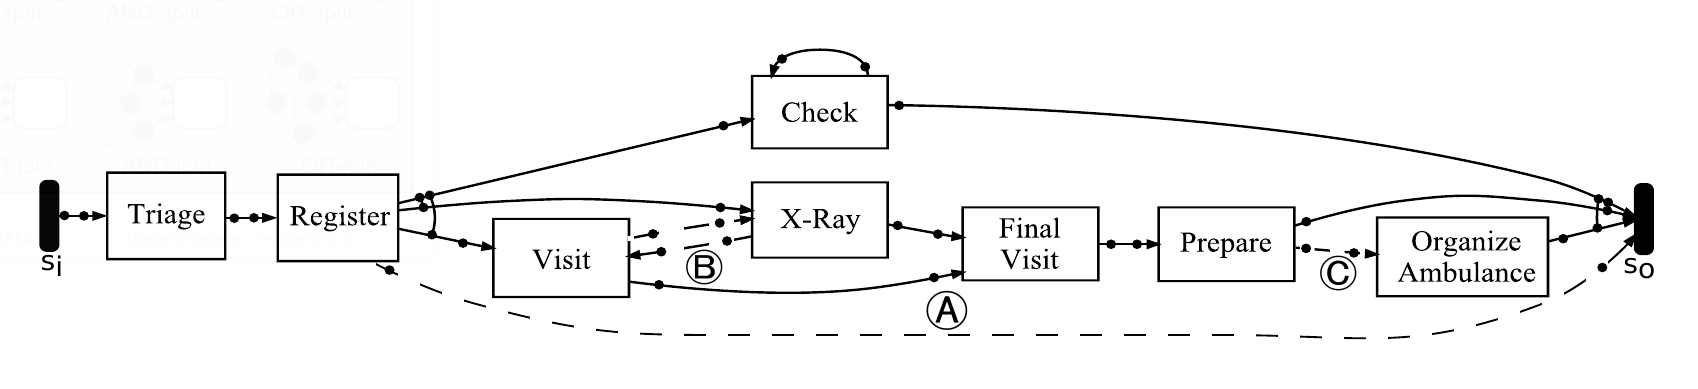
\includegraphics[width=1\textwidth]{Chapters/Graphics_Paper/C-net_ex_HB.jpg}
\caption{Synthetic Event Logs with 0\% Noise added\protect\cite{Mannhardt17}} 
\end{center}
\end{figure}

\begin{figure}[H]
\begin{center}
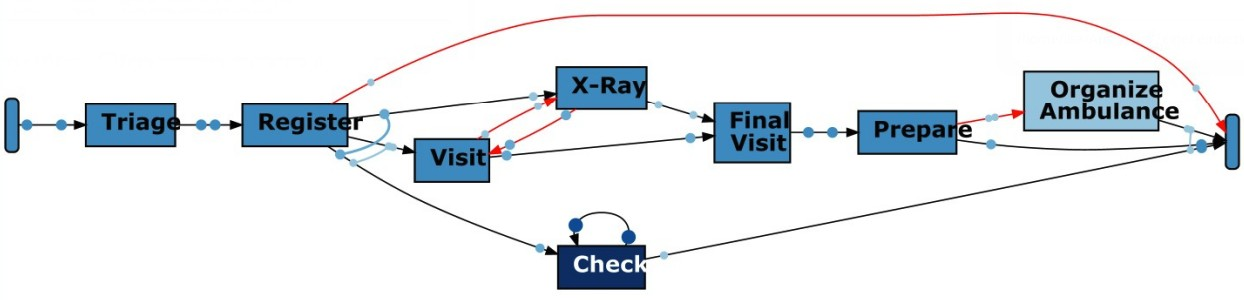
\includegraphics[width=0.9\textwidth]{Chapters/Graphics_Paper/Syn0NoiseReprod.jpg}
\caption{Reproduction - Synthetic Event Logs with 0\% Noise} 
\end{center}
\end{figure}



%----------------------------------------------------------------------------------------

\section{Hospital Billing}
\subsection{Evaluation design and set-up}
The Hospital Billing (HB) event log contains 100,000 cases with 550,000 events and 38 data attributes related to the billing of medical services.\\

\begin{table}[H]
\begin{tabularx}{\textwidth}
{>{\setlength\hsize{1\hsize}\setlength\linewidth{\hsize}}
X>{\setlength\hsize{1\hsize}\setlength\linewidth{\hsize}}
X>{\setlength\hsize{1\hsize}\setlength\linewidth{\hsize}}
X>{\setlength\hsize{1\hsize}\setlength\linewidth{\hsize}}
X>{\setlength\hsize{1\hsize}\setlength\linewidth{\hsize}}
X}
\textbf{Attributes} & & & \textbf{Methods} & \textbf{Thresholds} \\
\hline
\noindent
\begin{itemize}[leftmargin=*] 
\item CaseType
\item CloseCode
\item isClosed
\item Speciality

\end{itemize} &

\begin{itemize}[leftmargin=*] 
\item msgCode
\item msgType
\item isCancelled
\item version

\end{itemize} &
\begin{itemize}[leftmargin=*] 
\item blocked
\item flagA
\item flagB
\item flagC

\end{itemize} &
\begin{itemize}[leftmargin=*] 
\item DHM
\item HMF
\item IM
\end{itemize} &
\begin{itemize}[leftmargin=*] 
\item $\theta_{obs}$ = 0.04
\item $\theta_{dep}$ = 0.9
\item $\theta_{bin}$ = 0.001
\item $\theta_{con} \geqslant$ 0.6
\end{itemize}
\end{tabularx}
\end{table}



\noindent
Again the \textbf{accepted-task-connected heuristic} was used because not all of the 21 attributes are likely to be of interest. The \textbf{C4.5} was applied to 13 attributes and its performance was estimated using \textbf{10 times 10-fold cross validation}.\cite{Mannhardt2018b}

\subsection{Result comparison}

\begin{figure}[H]
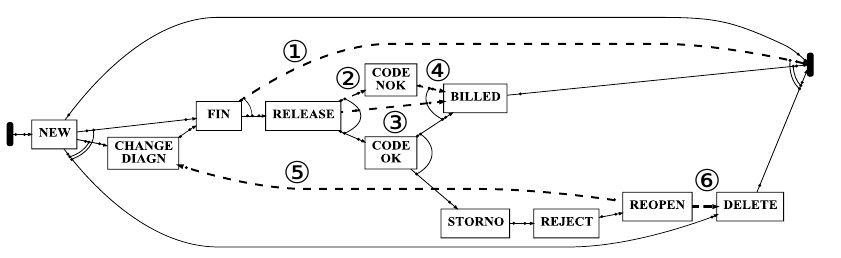
\includegraphics[width=1\textwidth]{Chapters/Graphics_Paper/HBresults.jpg}
\caption{Process model discovered by the authors \protect\cite{Mannhardt17}} 
\end{figure}

\begin{figure}[H]
\subfigure{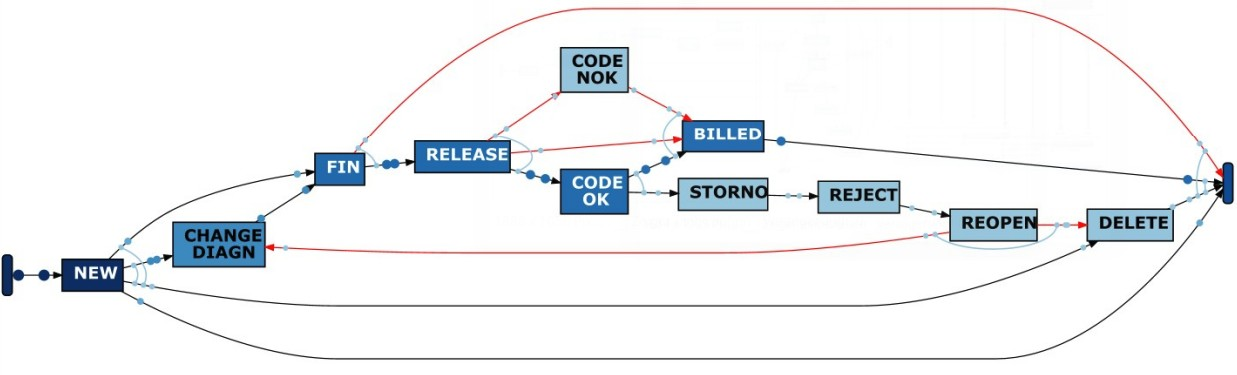
\includegraphics[width=0.9\textwidth]{Chapters/Graphics_Paper/HBreprod.jpg}}
\caption{Reproduced Process Model for the HB Event Logs} 
\end{figure}


%----------------------------------------------------------------------------------------

\section{Road Fines}
\subsection{Evaluation design and set-up}
The Road Fines (RF) event log contains about 150,000 cases, 500,000 events, and 9 data attributes.\\



\begin{table}[H]
\begin{tabularx}{\textwidth}
{>{\setlength\hsize{1.4\hsize}\setlength\linewidth{\hsize}}
X>{\setlength\hsize{1\hsize}\setlength\linewidth{\hsize}}
X>{\setlength\hsize{0.7\hsize}\setlength\linewidth{\hsize}}
X>{\setlength\hsize{0.9\hsize}\setlength\linewidth{\hsize}}
X}
\textbf{Attributes} & & \textbf{Methods} & \textbf{Thresholds} \\
\hline
\noindent
\begin{itemize}[leftmargin=*] 
\item isPaid
\item dismissal
\item paymentAmount
\item totalPaymentAmount
\end{itemize} &
\begin{itemize}[leftmargin=*] 
\item amount
\item points
\item article
\item expense
\end{itemize} &
\begin{itemize}[leftmargin=*] 
\item DHM
\item HMF
\item IM
\end{itemize} &
\begin{itemize}[leftmargin=*] 
\item $\theta_{obs}$ = 0.01
\item $\theta_{dep}$ = 0.8
\item $\theta_{bin}$ = 0.001
\item $\theta_{con} \geqslant$ 0.5
\end{itemize}
\end{tabularx}
\end{table}

\noindent
The \textbf{accepted-task-connected heuristic} was used and the \textbf{C4.5} was applied. Its performance was again estimated by the \textbf{10 times 10-fold cross validation}.

\subsection{Result comparison}

\begin{figure}[H]
\begin{center}
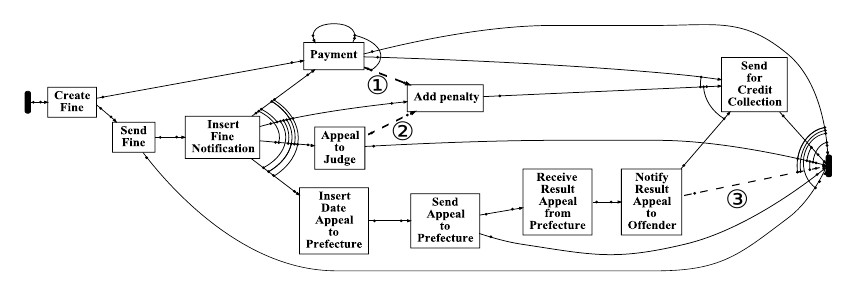
\includegraphics[width=1\textwidth]{Chapters/Graphics_Paper/RFresults.jpg}
\caption{Process model discovered for the RF Event Logs\protect\cite{Mannhardt17}} 
\end{center}
\end{figure}

\begin{figure}[H]
\begin{center}
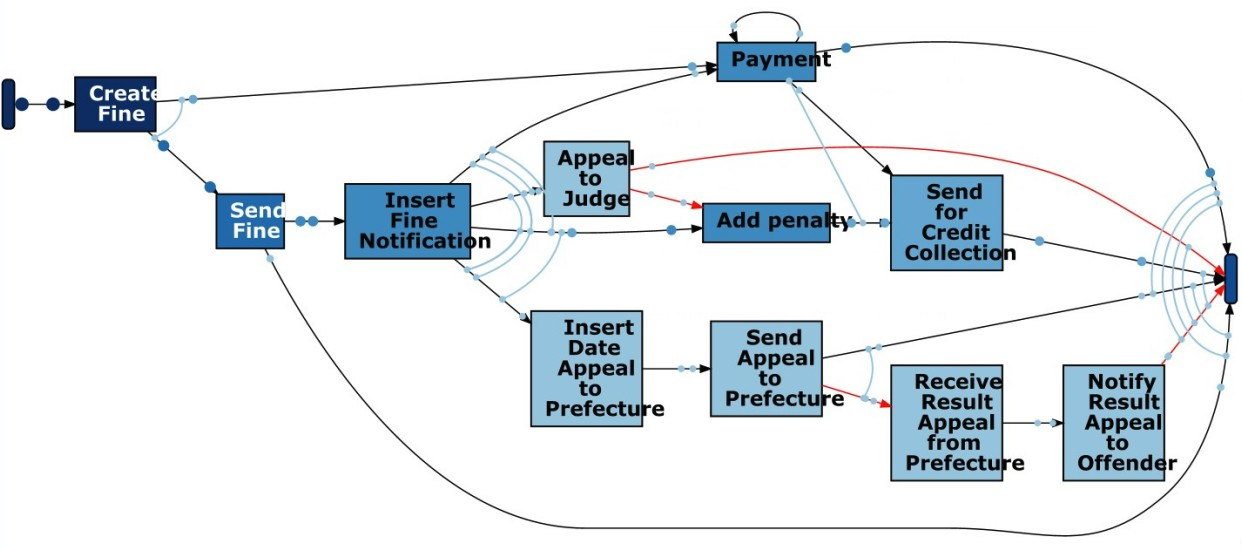
\includegraphics[width=0.9\textwidth]{Chapters/Graphics_Paper/RFreprod.jpg}
\caption{Result reproduction for the RF Event Logs} 
\end{center}
\end{figure}


 \section{Critical evaluation of the iDHM}